\documentclass[10pt,twocolumn]{article}
\usepackage[a4paper,margin=19mm,columnsep=7mm]{geometry}
\usepackage[T1]{fontenc}
\usepackage{lmodern,microtype,amsmath,amssymb,amsthm,booktabs,graphicx,xcolor,listings,xurl}
\usepackage[numbers,sort&compress]{natbib}
\usepackage[hidelinks]{hyperref}
\hypersetup{pdftitle={Valid JSON, Wrong Update: Preserving Field Presence in Agent Tool Calls},pdfauthor={Shivam Gupta}}
\usepackage{fancyhdr,titlesec}
\titlespacing*{\section}{0pt}{2ex plus .5ex minus .3ex}{1ex}
\titlespacing*{\subsection}{0pt}{1.7ex plus .4ex minus .2ex}{.8ex}
\titlespacing*{\paragraph}{0pt}{1.7ex plus .4ex minus .2ex}{.7em}
\pagestyle{fancy}\fancyhf{}\fancyhead[L]{\small Gupta | Presence-preserving agent interfaces}\fancyhead[R]{\small Technical research report}\fancyfoot[C]{\thepage}
\setlength{\headheight}{14pt}
\setlength{\emergencystretch}{1em}
\newtheorem{proposition}{Proposition}
\newtheorem{theorem}{Theorem}
\lstset{basicstyle=\ttfamily\scriptsize,breaklines=true,columns=fullflexible,frame=single,rulecolor=\color{black!20},showstringspaces=false}
\newcommand{\nul}{\mathsf{null}}
\newcommand{\abs}{\bot}
\newcommand{\PB}{\textsc{PresenceBridge}}
\title{Valid JSON, Wrong Update:\\Preserving Field Presence in Agent Tool Calls}
\author{Shivam Gupta\\Independent Researcher; Founder, Siloed\\\small\texttt{shivam1720406@gmail.com}}
\date{17 October 2026}
\begin{document}
\maketitle
\begin{abstract}
Strict structured generation can require every declared tool argument to be present. Replacing optional fields with required nullable fields is convenient, but cannot represent both omission and explicit null when the source interface distinguishes them. We study this conversion as a reversible-interface problem. For independent optional fields, an exact fibre characterization identifies the information lost by null filling; an observation with $c$ ambiguous null coordinates has $2^c$ valid source requests. A selective compiler uses null as an omission sentinel only outside the source value language and introduces explicit tags otherwise. Structural induction establishes round-trip fidelity on a stated schema fragment. A pinned census finds 76 optional fields with explicit null markers across GitHub request schemas; 62 accept null under an OpenAPI validator, spanning 37 operations. A Stripe comparison finds no such markers in its inspected scope. Installed SDK probes reproduce required-field conversion and show why post-parse unset tracking cannot reconstruct lost presence. Exhaustive SQLite-backed replay covers 5,460 Boolean update requests: both reversible codecs preserve every request, while each null-only policy preserves 1,092. An all-null initial state conceals every final-state error of the forward-null policy. Independent enumerations and nested tests verify the mechanism. The contribution is a bounded compiler and an evaluation protocol for adapter fidelity, rather than a new optional-value type or a claim of improved model reasoning.
\end{abstract}
\noindent\textbf{Keywords:} tool calling; structured generation; field presence; schema compilation; agent evaluation; API updates.\\
\textbf{Artifact:} \href{https://github.com/shi1720/presencebridge}{code, data, and reproducibility}.

\section{Introduction}
An agent is asked to change a customer's owner while leaving the customer's note unchanged. A source API accepts an omitted \texttt{note} to preserve its current value and accepts \texttt{note: null} to clear it. The generation interface requires both keys. An adapter fills the omitted note with null; validation succeeds; the backend clears the note. Alternatively, the adapter removes every null before dispatch, preserving the note but making an explicit clearing request impossible. The model may have selected the right operation in either case. The representation cannot communicate the necessary distinction.

This is a familiar data-modeling problem at a consequential integration boundary. JSON Schema separates presence from nullability \citep{jsonschema}; Protocol Buffers documents explicit presence \citep{protobuf}; Rust's double-option serialization distinguishes missing, null, and a value \citep{serde}. JSON Patch already supplies explicit operations \citep{jsonpatch}. The research question is therefore not whether a third state exists. It is how to verify and compile a source tool interface when a generation surface removes the ordinary missing-key channel.

The all-fields-required pattern is documented for strict structured generation \citep{strictdocs}. The boundary matters because strict generation and downstream validation solve different problems. Structured-output benchmarks evaluate constraint compliance, coverage, efficiency, and task quality \citep{geng2025,lu2025}. Tool-use systems connect model outputs to REST services \citep{restgpt}, and stateful benchmarks assess changes to an environment \citep{toolsandbox}. A source-to-wire converter sits between these evaluation surfaces. Validity against its output schema does not imply that it preserves the source request.

We ask three questions. \textbf{RQ1:} Under what conditions can a sentinel-filled representation recover field presence? \textbf{RQ2:} Can a compiler preserve presence while requiring every wire property, without tagging every optional field? \textbf{RQ3:} Which measurements reveal or conceal the resulting adapter errors?

Our contribution combines an exact collision analysis, a selective reference compiler, and reproducible engineering evidence. The central result is deliberately conditional: for the supported schema language, a checked codec recovers the exact source request. It does not establish whether a language model understood a user, whether a tool is authorized, or whether a service implements its published specification. The empirical contribution isolates representation from those additional uncertainties.

\section{Related work and scope of novelty}
\paragraph{Presence and update protocols.}
Missing-versus-null distinctions predate language models. JSON Merge Patch assigns null a removal meaning and consequently cautions about documents that use explicit null values \citep{mergepatch}. JSON Patch separates operations from values \citep{jsonpatch}. Protocol Buffers describes how implicit presence can prevent default-valued fields from participating in merge operations \citep{protobuf}. The \texttt{serde\_with} double-option adapter preserves three states through ordinary JSON \citep{serde}. These are substantive antecedents: neither an explicit tag nor the distinction being preserved is new here. Our compiler adapts those principles to an all-fields-required generation profile and makes the selective tagging criterion executable.

\paragraph{Schemas and structured generation.}
Formal work gives JSON Schema a language-theoretic treatment \citep{pezoa2016}. JSONSchemaBench evaluates real schemas, including over- and under-constraining behavior \citep{geng2025}; SchemaBench and schema reinforcement learning study output validity and downstream performance \citep{lu2025}. Our object of evaluation is a pair of languages and their adapter, rather than output membership in one language. We complement those measurements with $D(E(x))=x$, exact request comparison, and backend-state replay. We do not claim that existing benchmarks universally ignore semantics.

\paragraph{Tool execution and serialization.}
RestGPT makes parameter formulation part of a REST executor \citep{restgpt}. BFCL evaluates function-calling capabilities \citep{bfcl}, while ToolSandbox evaluates stateful trajectories and milestones \citep{toolsandbox}. Pydantic tracks explicitly supplied fields and supports both unset-based and null-based exclusion \citep{pydantic}. Those facilities preserve distinctions present in the parsed input; they cannot recreate a distinction already collapsed by the wire encoding. We test that specific boundary in installed, unmodified libraries.

\paragraph{What is new in this study.}
The work contributes a connected artifact: a precise sentinel-collision test, a compiler that introduces tags selectively, a two-provider source audit with a negative control, and an exhaustive state-coverage counterexample. The proofs are elementary and expose assumptions; they are not presented as new information theory or a new sum type. Our literature search covered primary structured-generation papers, stateful tool benchmarks, update standards, presence-aware serializers, provider documentation, and SDK source. It did not establish patent novelty or the absence of every prior implementation. The appropriate positioning is a reproducible systems study for engineers deploying agent interfaces.

\section{Problem formulation}
Let $S$ be a source schema and $L(S)$ its valid JSON values. At an object node, a field $i$ has a set $V_i$ of accepted present values. If the field is optional, its states are $V_i\cup\{\abs\}$, where $\abs$ denotes omission and is distinct from JSON null. A required field has states $V_i$. We initially assume independent fields: there are no cross-field dependencies, conditionals, or constraints that couple which keys may be omitted.

For a wire encoder $E$ and decoder $D$, \emph{request fidelity} means
\begin{equation}\label{eq:roundtrip}
  \forall x\in L(S),\quad D(E(x))=x.
\end{equation}
Equality here preserves keys, JSON types, array order, and values; object-key order is immaterial. A deterministic backend $F(s,x)$ maps initial state $s$ and request $x$ to its outcome. Equation~\ref{eq:roundtrip} implies
\begin{equation}
 F(s,D(E(x)))=F(s,x)
\end{equation}
for identical execution context. The converse need not hold for a restricted state set. Clearing an already-null field and leaving it unchanged can yield the same final record despite different requests.

Define null filling $N$ by replacing every optional omission with null and otherwise leaving field values unchanged. Required fields are retained. For a wire observation $y$, define
\begin{equation}
 C(y)=\{i:\ i\text{ optional},\ \nul\in V_i,\ y_i=\nul\}.
\end{equation}
Only observations in the image of $N$ are considered. A nullable required field is not ambiguous; an optional nonnullable field's null is unambiguously the omission sentinel.

\begin{proposition}[Exact collision size]\label{prop:fibre}
For independent fields, $|N^{-1}(y)|=2^{|C(y)|}$. Hence no decoder using $y$ alone satisfies request fidelity when $C(y)$ is nonempty. A fixed-width auxiliary binary message distinguishing all preimages of this particular $y$ requires at least $|C(y)|$ bits in the worst case, and that bound is attainable.
\end{proposition}
\begin{proof}
Every coordinate outside $C(y)$ has exactly one source state: a present non-null value, a required null, or an omitted optional nonnullable field. Each coordinate in $C(y)$ independently has two source states, omission and explicit null. Multiplication gives the fibre size. A decoder must choose one output for $y$ and therefore cannot recover all members of a non-singleton fibre. A fixed-width binary message with fewer than $|C(y)|$ bits has fewer than $2^{|C(y)|}$ possible values. Conversely, one presence bit for each ambiguous coordinate distinguishes every member. This is an information bound, not a claim about JSON token optimality.
\end{proof}

The same criterion holds for any sentinel $a$: mapping omission to $a$ collides exactly when $a\in V_i$ for an optional field. Replacing null with the empty string, zero, false, an empty array, or a source-accepted default merely relocates the collision. An explicit presence list, a bit channel, or an operation tag restores information. Those alternatives may differ in decoder complexity and generation cost.

\section{The PresenceBridge compiler}
\subsection{Supported schema language}
The implementation accepts finite-tree, closed objects with named properties and a required-key set; homogeneous arrays; explicit scalar types; nullable single-type variants; scalar \texttt{enum}/\texttt{const}, numeric bounds and multiples, string length and pattern constraints, and array length constraints. It normalizes a single type-or-null \texttt{anyOf}. It rejects references, open maps, arbitrary unions, dependencies, conditional schemas, formats, and unrecognized validation keywords. Metadata such as \texttt{title} and \texttt{default} is removed from the compiled language; JSON Schema defaults are annotations, and backend defaulting remains the backend's responsibility after omission is recovered.

This boundary is essential. The census examines a larger OpenAPI surface and does not establish that every audited endpoint is compilable by this prototype. OpenAPI~3.0 \texttt{nullable} is interpreted for the census; the codec itself accepts the documented JSON Schema fragment. Unsupported inputs fail at construction rather than receiving an approximation.

\subsection{Selective encoding}
Let $\widehat V$ denote the recursively compiled representation of a present value. Required fields retain that representation. An optional nonnullable field uses null for omission and $\widehat V$ for a present value. An optional nullable field uses a disjoint tagged union:
\begin{lstlisting}
{"op":"omit"}
{"op":"set","value": <compiled source value>}
\end{lstlisting}
The \texttt{set} branch may contain explicit null. Each branch is a closed object whose declared properties are all required. The outer object also requires every declared property. The full-tag baseline uses the same union for every optional field, including nonnullable fields. Required fields are never unnecessarily wrapped.

For example, a source interface with optional nonnullable \texttt{enabled} and optional nullable \texttt{note} can encode ``leave enabled alone; clear note'' as
\begin{lstlisting}
{
  "enabled": null,
  "note": {"op":"set","value":null}
}
\end{lstlisting}
The decoded source request is exactly \texttt{\{"note":null\}}. A source value containing keys named \texttt{op} or \texttt{value} cannot impersonate the wrapper because it resides inside the wrapper's \texttt{value} member.

\begin{theorem}[Round-trip fidelity]\label{thm:codec}
For every schema in the supported language and every valid source value $x$, both implemented codecs satisfy Equation~\ref{eq:roundtrip}. Their compiled object nodes are closed and require every declared property.
\end{theorem}
\begin{proof}
Proceed by structural induction. Scalars and null preserve their values. For arrays, the inductive hypothesis applies elementwise, preserving order and length. At an object node, required fields use the inductive hypothesis directly. An optional nonnullable field is absent exactly when its wire value is null; a present value cannot encode as null because its source schema excludes null and recursive compilation preserves a non-null value's outer JSON kind. An optional nullable field's disjoint \texttt{omit} and \texttt{set} branches explicitly identify absence; the latter recovers its value by induction, including null. The full-tag baseline applies this last argument to every optional field. Reconstruction preserves all and only source keys. The compiler explicitly sets every object node's required list to its property names and closes both ordinary objects and tag variants.
\end{proof}

The public encoder validates the source and its compiled result. The public decoder validates the wire input, reconstructs the source, and validates the reconstruction. No coercion is applied. This checks a representation contract; authorization and business invariants still belong at the execution boundary. The theorem does not promise hosted-provider support for every copied scalar constraint. We test local schema behavior and installed SDK transformations, not acceptance by a remote decoder service.

\subsection{Cost and alternatives}
For a finite schema tree, the compiler adds constant-sized structure per optional field; schema size is linear in the input size absent pre-existing duplication. Excluding validator-specific costs and scalar-predicate evaluation, encoding and decoding perform one structural visit to each traversed value node and declared property. Arrays retain their order. Full tags and JSON Patch provide explicit alternatives; direct passthrough remains preferable when the generation surface supports optional keys. Our selective strategy is a conservative engineering choice, not a universal minimum-token encoding. A bitmap can be more compact but introduces an additional alignment contract. We measure two tokenizers rather than infer cost from wrapper count.

\section{Empirical protocol}
All experiments isolate the adapter. Source requests are deliberately constructed or enumerated, not sampled from model outputs. Consequently the study can establish a deterministic failure mechanism and verify a reference implementation, but cannot estimate deployed failure prevalence or changes in model task success.

\paragraph{Public source census.}
We freeze GitHub's official REST description at commit \texttt{0fa95c50cd6f} and Stripe's official OpenAPI description at \texttt{4d2b98a2a17f} \citep{githubspec,stripespec}. The artifact records complete commits, SHA-256 hashes, retrieval URLs, and field-level evidence. Both are commercially consequential, public machine-readable APIs; they were selected purposively, not randomly.

We enumerate eight standard HTTP method keys, resolve local references at the request-body root and each inspected field, prefer JSON media when available, otherwise inspect form encoding, and count each operation once. We inspect top-level properties only. A null marker is an explicit declaration through \texttt{nullable}, a null type, or a union containing an explicitly nullable branch. We do not infer nullability from an unspecified type. For optional marked fields, we independently validate null with the pinned OpenAPI~3.0 validator \citep{oasvalidator}. This matters because other constraints can still reject null \citep{oas}. We retain rejection keywords and count an accepted exposure only when null passes that validator. Union-only roots and unsupported media do not enter the field denominator. We report these exclusions. This measures representational exposure, not server execution or intent.

\paragraph{SDK and hydration probes.}
Unmodified OpenAI Python~3.33.0 and Agents SDK~0.24.0 convert Pydantic~2.14.1 model schemas \citep{sdk,agents}. We save input and output schemas, package versions, and source-file hashes. A nullable model with defaults allows omitted source fields; strict conversion requires both properties. We compare Pydantic's field-set metadata and \texttt{exclude\_unset}/\texttt{exclude\_none} on omitted and explicitly null inputs. A separate non-null-default model is retained as a conversion control. No hosted API is called, and a retained \texttt{default} annotation is not treated as proof of remote acceptance.

\paragraph{Exhaustive effect replay.}
For $n=1,\ldots,6$ optional nullable Boolean fields, enumerate all $4^n$ vectors from omission, null, true, and false. This yields $\sum_{n=1}^{6}4^n=5{,}460$ source requests. The independent oracle stores the initial record in SQLite and updates only explicitly supplied source keys. Each initial field is true, so omission and clearing have distinct outcomes. We compare null filling followed by (i) forwarding every null, (ii) dropping every null, (iii) selective decoding, or (iv) full-tag decoding. The first two are explicit experimental policies, not undocumented SDK defaults. We also replay forwarding against an initially all-null record as a masking control. Per-case data include exact request and final-state agreement.

\paragraph{Verification and cost.}
An independent tuple enumerator groups normalized requests into fibres for $n=1,\ldots,7$ and checks Proposition~\ref{prop:fibre}. It separately enumerates initially null-or-true records and source requests for $n=1,\ldots,5$. The codec suite exhausts Boolean vectors through five fields, adds 2,000 generated nested round trips across two codecs with 20 fixed seeds, and rejects malformed tags, mistyped source values, extra keys, and unsupported schemas.

The token benchmark enumerates all valid patches for four fixed Boolean field names with zero, two, or four nullable fields: 81, 144, and 256 source requests. Compact UTF-8 JSON is tokenized with \texttt{cl100k\_base} and \texttt{o200k\_base} using tiktoken~0.14.0. We measure source passthrough, null filling, selective tags, and full tags on the same requests. These counts exclude prompts, schemas, reasoning, and retries; they are payload costs, not total inference costs. No confidence intervals are attached to exhaustive finite populations.

\section{Results}
\subsection{Where the source distinction occurs}
Table~\ref{tab:census} separates total operations from the request-object population. GitHub contributes 76 optional fields with null markers among 1,250 inspected fields (6.08\%). Of these, 62 accept null under the OpenAPI validator (4.96\% of inspected fields), spanning 37 of 332 inspected object operations (11.14\%). Fourteen marked fields reject null: ten through \texttt{enum} and four through \texttt{oneOf}. Thus counting nullable markers alone would overstate validator-confirmed exposure. This is a schema-layer discrepancy, not a verified production-service bug. Nineteen of its 74 PATCH operations have a detected exposure. Stripe contributes zero explicit nullable exposures among 2,278 inspected fields. Its zero result is meaningful for this declared null audit: Stripe also uses other clearing conventions, including empty values \citep{stripeapi}. It is not evidence that Stripe updates need no presence tracking.

\begin{table}[t]
\centering\small
\begin{tabular}{lrr}
\toprule & GitHub & Stripe\\\midrule
All operations & 1,242 & 612\\
Operations with request body & 352 & 612\\
Inspected object operations & 332 & 611\\
Union/non-property roots skipped & 18 & 0\\
Other media excluded & 2 & 1\\
Inspected top-level fields & 1,250 & 2,278\\
Optional fields & 946 & 2,109\\
Optional with null marker & 76 & 0\\
Marked null accepted / rejected & 62 / 14 & 0 / 0\\
Operations with accepted exposure & 37 & 0\\
PATCH operations / exposed & 74 / 19 & 0 / 0\\
\bottomrule
\end{tabular}
\caption{Pinned OpenAPI census. Exposures are schema declarations, not observed backend failures. Stripe's inspected form-encoded bodies are counted once per operation.}\label{tab:census}
\end{table}

A concrete source-level example is GitHub Pages' custom-domain field: the official interface documents null as removing the domain \citep{githubpages}. Other audit rows explicitly describe clearing a secret-alert assignee; the validity-override row also illustrates that prose permitting null can coexist with a null-rejecting enum. These examples motivate the distinction, but we do not execute destructive production calls. Some fields have context-dependent effects or required-by-description conditions; those remain outside our independence model. The inventory retains descriptions to make these limitations inspectable.

\subsection{What the installed stack preserves}
Both tested converters mark every declared property required. For the two-field nullable model, Pydantic records an empty field set for \texttt{\{\}}, but both fields as supplied for \texttt{\{"note":null,"owner":null\}}. Serializing the latter with \texttt{exclude\_unset=True} retains both nulls; \texttt{exclude\_none=True} removes both. Neither policy distinguishes a null standing for omission from a null standing for an explicit clear. This is expected from the information available, not a failure of Pydantic's documented unset tracking. It also does not show that the SDK itself implements a particular null-to-omission policy.

\subsection{Request fidelity and effect fidelity}
Both reversible codecs recover all 5,460 source requests. Either null-only policy recovers $\sum_{n=1}^{6}3^n=1{,}092$ requests (20.00\%) and produces the correct final state for those same requests when every initial value is true. At six fields, the result is 729/4,096 (17.80\%), compared with 4,096/4,096 for each codec (Figure~\ref{fig:effects}). The exact failure fraction reflects exhaustive, equally weighted constructed states; it is not a prediction of production traffic.

\begin{figure*}[t]
\centering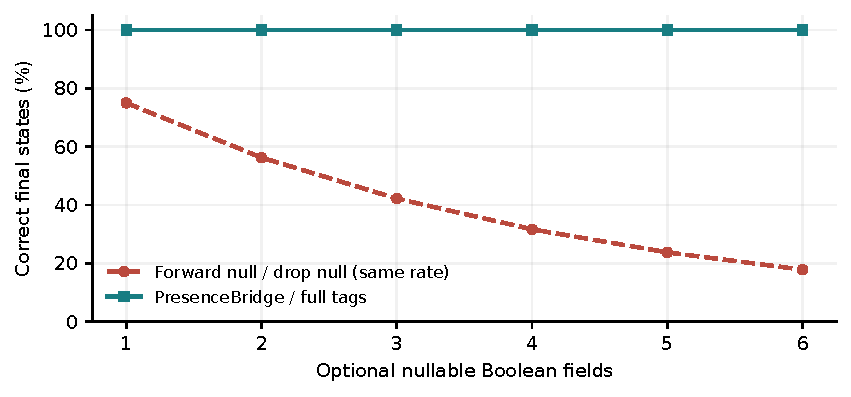
\includegraphics[width=.87\textwidth]{effects.pdf}
\caption{Exact final-state agreement on exhaustive optional-nullable Boolean updates. Every initial field is true. The two null-only policies have the same rate, $(3/4)^n$, but fail on different requests: forwarding null damages omissions, while dropping null loses explicit clears. Both reversible codecs preserve all requests.}\label{fig:effects}
\end{figure*}

\begin{proposition}[State-coverage masking]\label{prop:mask}
For $n$ independently and uniformly selected source states from omission, null, true, and false, fix an initial record with $k$ non-null fields. Either null-only policy has final-state agreement $(3/4)^k$. If initial fields are independently null with probability $p$, expected agreement is $(1-(1-p)/4)^n$.
\end{proposition}
\begin{proof}
For forwarding, a non-null initial field differs from the intended outcome precisely when the source omits it: one of four states. For dropping null, it differs precisely when the source explicitly supplies null. At an initially null field, either event leaves the same final value as the oracle, and non-null supplied values are retained. Independence gives $(3/4)^k$. Averaging one field over its initial state gives $p+(1-p)3/4$ and multiplication gives the stated expression.
\end{proof}

The all-null control has perfect final-state agreement for every forwarded request, while exact request agreement remains 1,092/5,460. Thus the same lossy representation can score 100\% or 20\% under a change only to the evaluator's starting state. The independent enumerator verifies all 124 state-policy configurations through five fields. Figure~\ref{fig:mask} plots the analytical expectation; it is not a fitted empirical curve. Operationally, evaluation needs separating states: for each omission/clear pair, include a permitted state where their outcomes differ. If no such state exists in the declared backend context, the pair is observationally equivalent there, and exact presence is a stronger requirement than that context's final-state objective.

\begin{figure*}[t]
\centering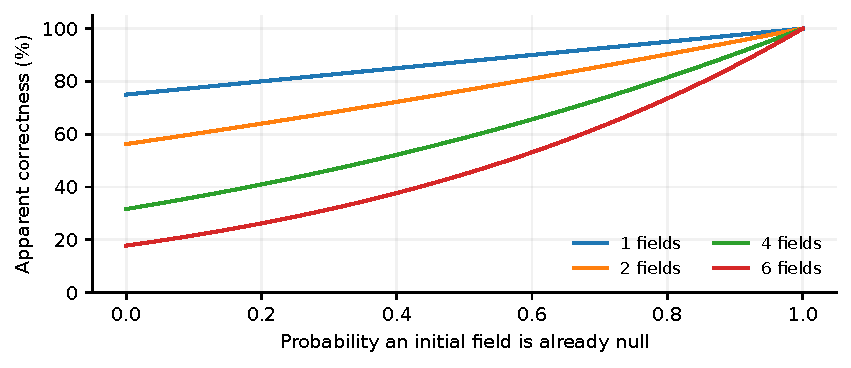
\includegraphics[width=.87\textwidth]{state_masking.pdf}
\caption{Analytical effect of the evaluator's initial-state distribution (Proposition~\ref{prop:mask}). Increasing the probability that fields already contain null inflates apparent adapter correctness without restoring a single lost request distinction.}\label{fig:mask}
\end{figure*}

\subsection{Checks and representation cost}
The independent checker verifies 3,279 normalized fibres, all with the predicted size. The 26-test codec suite passes, including nested arrays and objects, nullable container values, required nulls, malformed tags, and source-type rejection. This supports the implementation on the stated fragment; it does not substitute for a proof or cover arbitrary JSON Schema. The validation-inclusive encode/decode probe records a median 357.15~$\mu$s and 95th percentile 543.75~$\mu$s over 10,920 measured pairs in Python~3.12.14 on macOS~27.0.1/arm64. This single-process observation is not a latency SLA or a comparison with hosted inference.

Selective tagging reduces mean payload tokens relative to full tagging when some optional fields exclude null (Table~\ref{tab:tokens}, Figure~\ref{fig:tokens}). With two nullable fields, the reduction is 25.0\% for \texttt{cl100k\_base} and 25.3\% for \texttt{o200k\_base}. When every optional field is nullable, the encodings coincide and there is no advantage. Null filling is smaller but cannot preserve all source states in that condition. Savings depend on names, value distributions, tokenizer, and wire design; these results establish an example tradeoff rather than universal token dominance.

\begin{table}[t]
\centering\small
\begin{tabular}{llrrr}
\toprule Tokenizer & Encoding & $c=0$ & $c=2$ & $c=4$\\\midrule
\texttt{cl100k} & Null fill & 18.00 & 18.00 & 18.00\\
 & Selective & 18.00 & 28.00 & 38.00\\
 & Full tags & 36.67 & 37.33 & 38.00\\\midrule
\texttt{o200k} & Null fill & 18.00 & 18.00 & 18.00\\
 & Selective & 18.00 & 28.50 & 38.75\\
 & Full tags & 37.67 & 38.17 & 38.75\\\bottomrule
\end{tabular}
\caption{Mean compact payload tokens. Here $c$ denotes the number of nullable fields in the four-field schema, rather than the observation-specific collision count of Proposition~\ref{prop:fibre}. All optional fields are nonnullable when $c=0$.}\label{tab:tokens}
\end{table}

\begin{figure*}[t]
\centering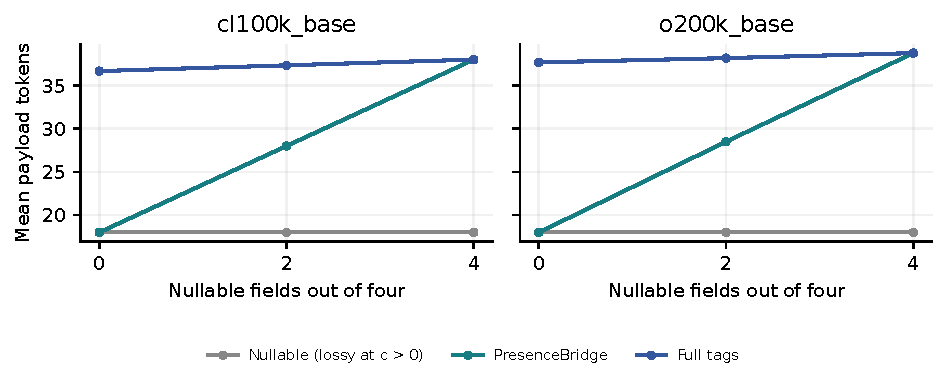
\includegraphics[width=.87\textwidth]{tokens.pdf}
\caption{Payload-cost tradeoff on four named Boolean fields. Full enumeration covers 81, 144, and 256 requests at zero, two, and four nullable fields. Source passthrough is retained in the artifact but omitted here because it uses the missing-key channel unavailable in the stipulated strict profile.}\label{fig:tokens}
\end{figure*}

\section{Engineering and commercial implications}
Presence fidelity belongs in a tool adapter's regression suite. A useful suite has three layers: validate source and compiled schemas; test exact request round trips; and replay operations from states that distinguish omission from explicit changes. Checking only syntactic validity can miss representation loss. Checking only final state can also miss it when fixtures begin at a default value.

For a customer-support agent, this contract prevents an unchanged field from becoming a clear operation during conversion. For configuration assistants, it separates inheritance from an explicit default-valued override. For developer tools, it distinguishes preserving a setting from disabling or removing it. These are plausible applications of the verified mechanism, not measured customer outcomes. The practical product opportunity is an auditable integration layer: schema admission, compatibility diagnostics, reversible codecs, and replayable migration checks. A commercial deployment would still need provider-specific schema admission, access control, versioning, observability, and workload-specific evaluation.

The evidence does not establish a defensible patent claim. The underlying presence types, tags, and explicit update protocols have substantial prior art. A more credible value proposition is reliable implementation and integration coverage, rather than exclusivity over the basic encoding. The open artifact makes the contract reviewable and allows teams to compare it with direct optional-key output or JSON Patch before adopting another wire format.

\section{Limitations and threats to validity}
\paragraph{Novelty and generalization.}
The contribution is a bounded engineering study. The collision argument follows elementary injectivity and counting. Presence-aware serialization is established. Two purposively chosen API descriptions cannot estimate industry prevalence. The census omits nested fields, some media, and union-only roots; repeated field uses are counted as distinct operation-field slots. Even validator-confirmed null acceptance does not prove that omission and null have different runtime effects.

\paragraph{Model behavior and provider support.}
We do not run a language-model comparison. A more expressive wire language may be harder for a model to use, and larger schemas may increase prompt or decoding cost. Structural round-trip fidelity cannot guarantee semantic selection, completion, correct value extraction, or authorization. The implementation uses a profile with closed, all-required objects, but hosted engines can support different schema keywords and complexity limits. A production admission check must be tested against its chosen engine.

\paragraph{Backend and evaluation assumptions.}
The replay backend implements a simple partial-update contract; it is not a live GitHub or Stripe server and does not model triggers, races, access checks, or cross-field requirements. Exact request equality is intentionally stronger than final-state equality. Some APIs treat omission and null identically for particular fields or states, reducing the need for a presence channel there. Our four-state construction weights all possibilities equally to expose a failure mechanism; production weighting could yield a much smaller or larger error rate.

\paragraph{Implementation and cost.}
The compiler rejects general references, recursive schemas, arbitrary unions, and conditional constraints. Expanding its language requires new proof cases and differential tests. Regex validation costs and library recursion limits are outside its structural complexity statement. Payload token savings do not include schema tokens, retry rates, caching, or latency. Measurements and source snapshots are version-specific; the artifact records their precise environment and hashes.

\section{Conclusion}
Strict schema compliance can coexist with irreversible loss of a source action distinction. Null filling is reversible for an optional field precisely when null is excluded from its present-value language; otherwise an additional presence channel is necessary. \PB{} makes that criterion executable with selective tags, while exact request comparison and separating backend states reveal errors that default-valued fixtures can conceal. The result is a reproducible adapter contract and test methodology for tool-using systems, with explicit boundaries on schema coverage, model behavior, and deployment claims.

\section*{Artifact and reproducibility}
The repository contains the compiler, pinned dependencies, 26-test suite, API-source manifest and field inventory, exhaustive effect rows, independent fibre/state checker, tokenizer measurements, figure scripts, and this manuscript's \LaTeX{} source. All stated numerical results are generated from saved experiment outputs. Public API documents are re-fetched from pinned commits and checked by hash; production APIs are not modified. Appendix~\ref{app:commands} gives execution commands. The artifact is released under MIT for original code; upstream specifications retain their own licenses.

\bibliographystyle{plainnat}
\bibliography{references}
\appendix
\section{Reproduction commands and artifact map}\label{app:commands}
Use Python~3.12 and a fresh virtual environment. The frozen lock records exact experiment dependencies. Install the package after the lock and run:
\begin{lstlisting}
python -m pip install -r requirements-lock.txt
python -m pip install -e .
python -m pytest -q
python experiments/audit.py
python experiments/benchmark.py
python experiments/verify.py
python experiments/figures.py
cd paper
tectonic main.tex
\end{lstlisting}
\texttt{audit.py} downloads only pinned public descriptions into an ignored cache. The hash manifest is \texttt{data/sources.json}; the request-slot evidence is \texttt{data/field\_inventory.csv}. \texttt{benchmark.py} regenerates effect and token rows, SDK probes, and the environment report. \texttt{verify.py} imports no codec code and checks tuple transitions independently. \texttt{figures.py} reads saved results and regenerates the three vector figures. Runtime timings can vary; exhaustive counts and token totals should match.

\end{document}
